\section{Sistem ve Kanal Modeli}
\label{sec:system}

\subsection{Sinyal Modeli}
Yarım dalga boyu aralıklı $N_t=8$ antenden oluşan düzgün doğrusal diziye sahip bir baz istasyonu (BS), $K=4$ tek antenli kullanıcıya doğrudan bir bağlantı ve $N=32$ pasif elemanlı bir RIS ($8\times 4$ düzlemsel dizi) üzerinden hizmet verir; Bölüm~\ref{sec:res_scaling} ayrıca $N=64$ durumunu da kullanır. Fazlar $\bs{\theta}\in[0,2\pi)^N$, $\mbf{v}=e^{j\bs{\theta}}$ ve ön kodlayıcı $\mbf{W}=[\mbf{w}_1,\dots,\mbf{w}_K]$ olmak üzere, $k$ kullanıcısı şu sinyali alır:
\begin{equation}
    y_k = \left(\mbf{h}_{d,k}^H + \mbf{g}_k^H \operatorname{diag}(\mbf{v})\mbf{F}\right)\sum_{j=1}^K \mbf{w}_j s_j + n_k ,
    \label{eq:signal}
\end{equation}
burada $\mbf{F}\in\mathbb{C}^{N\times N_t}$ BS--RIS kanalı, $\mbf{g}_k^H$ RIS--kullanıcı kanalı, $\mbf{h}_{d,k}^H$ doğrudan kanaldır ve gürültü $n_k\sim\mathcal{CN}(0,\sigma^2)$ biçimindedir. Parantez içindeki etkin kanal $\mbf{h}_k^H(\bs{\theta})$ ile gösterildiğinde, $k$ kullanıcısının hızı $R_k=\log_2(1+\mathrm{SINR}_k)$ olur; burada sinyal-girişim-artı-gürültü oranı $\mathrm{SINR}_k = |\mbf{h}_k^H \mbf{w}_k|^2/(\sum_{j\ne k}|\mbf{h}_k^H \mbf{w}_j|^2 + \sigma^2)$ biçimindedir. Ön kodlayıcı, etkin kanal üzerinde düzenlileştirilmiş sıfır zorlamadır (ZF)~\cite{Peel2005TCOM}; düzenlileştirici $\lambda = K\sigma^2/P$ ve toplam güç $P$ olarak alınır. Amaç fonksiyonu en düşük kullanıcı hızıdır; bu, RIS destekli çok girişli tek çıkışlı (MISO) sistemler için~\cite{Nadeem2020TWC} çalışmasında da kullanılan bir adalet ölçütüdür:
\begin{equation}
    \max_{\bs{\theta}} \; \min_k R_k(\bs{\theta}),
    \label{eq:maxmin}
\end{equation}
Adam, Armijo ve öğrenilen güncelleme (Bölüm~\ref{sec:method}) bu problemi pürüzsüz vekil $-\tfrac{1}{\beta}\log\sum_k e^{-\beta R_k}$, $\beta=8$ üzerinden optimize eder; koordinat inişi ve uzun koşulu Adam referansı ise katı minimumu maksimize eder.

\subsection{Geometri ve Yayılım}
\begin{figure*}[t]
\centering
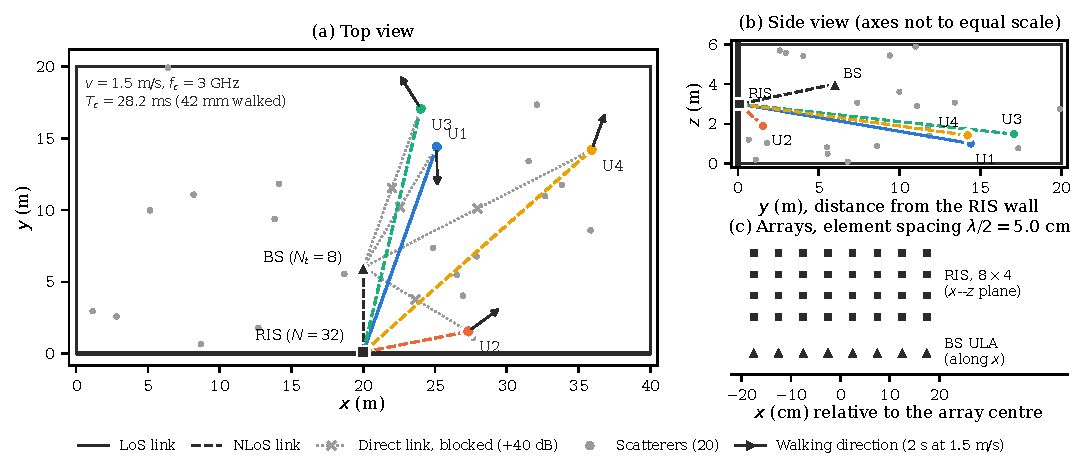
\includegraphics[width=\textwidth]{figures/fig_scenario.pdf}
\caption{Benzetimi yapılan senaryo (eskime kümesinin ilk senaryosu). (a)~$40\times20\times6$~m boyutlu ofisin üstten görünümü: BS $(20,6,4)$~m konumunda, duvara monte edilmiş RIS $(20,0.1,3)$~m merkezli, 1.5~m/s hızla yürüyen dört kullanıcı, 20 noktasal saçıcı. Çizgi stili: her bağlantının görüş hattı (LoS) durumu. Bütün doğrudan bağlantılar 40~dB'lik engellemeyi taşır. Oklar: 2~s'lik yürüyüş; bir eş evrelilik süresi içinde bir kullanıcı yalnızca 42~mm yer değiştirir. (b)~Yandan görünüm. (c)~Eleman yerleşimleri.}
\label{fig:scenario}
\end{figure*}
Oda $40\times 20\times 6$~m boyutundadır (Şekil~\ref{fig:scenario}). RIS bir duvar üzerinde $(20, 0.1, 3)$~m noktasında merkezlenmiştir; BS ise $(20, 6, 4)$~m noktasında, panelin bakış ekseni (boresight) üzerinde ve panelin Fraunhofer uzaklığının ötesindedir. Kullanıcılar 1--2~m yüksekliklere düzgün dağılımla yerleştirilir. Taşıyıcı frekansı $f_c=3$~GHz, bant genişliği 20~MHz, iletim gücü 20~dBm, BS anten kazancı 5~dBi ve gürültü faktörü 7~dB'dir. Bütün bağlantılar 3GPP TR~38.901 iç mekân ofis modelini~\cite{3gpp_channel} izler: bu modelin yol kaybı, karma ofis LoS olasılığı, Rician faktörü ve 5~m'de üstel uzamsal korelasyonlu log-normal gölgelemesi (TR~38.901, LoS için 10~m, görüş hattı dışı (NLoS) için 6~m öngörür). NLoS bileşenleri, bir senaryonun bütün bağlantılarınca paylaşılan noktasal saçıcılardan gelir. Kademeli (cascaded) genlik, $\cos^q$ güç örüntülü ($q{=}1$) serbest uzay iki atlamalı modeli~\cite{Tang2021TWC} izler; her atlamaya TR~38.901 ek kaybını ve gölgelemesini ekliyoruz. Bizim eleman kazancımız $2(2q{+}1)$, Tang'in $2(q{+}1)$ kazancını aşar; ikincisi mutlak hızları yaklaşık \%5 düşürür ve $L^\star$ ile en iyi yöntemi değiştirmez. RIS, doğrudan yolun engellendiği yerlere konuşlandırıldığı için doğrudan bağlantı fazladan 40~dB kayıp taşır.

\subsection{Hareketlilik}
Kullanıcılar $v=1.5$~m/s (5.4~km/h) hızla düz çizgiler boyunca yürür ve duvarlardan yansır. Bu değer, 3GPP iç mekân sıcak nokta değerlendirmesindeki 3~km/h~\cite{3gpp_tr38913} ile iç mekân hareketliliğinin değerlendirildiği IMT-2020 yaya sınıfının 10~km/h üst sınırı~\cite{itu_m2410} arasında yer alır; Bölüm~\ref{sec:res_sensitivity} ana ölçümleri bu hızlarda ve daha yüksek hızlarda tekrarlar. Saçıcılar, yol kazançları, LoS durumları, gölgeleme ve $\mbf{F}$ sabit tutulur; yalnızca kullanıcılar hareket eder ve $\mbf{g}_k(t)$ ile $\mbf{h}_{d,k}(t)$ her anda geometriden yeniden hesaplanır. Referans zaman ölçeği Doppler frekansı $f_d=vf_c/c=15$~Hz'dir; buna karşılık gelen eş evrelilik süresi $T_c=\sqrt{9/(16\pi)}/f_d\approx0.423/f_d=28.2$~ms'dir.

\emph{Sınırlamalar.} Sabit saçıcılar, kanalın saniyeler mertebesinde gerçek bir kanaldan daha az değişmesine yol açar; bu nedenle 200~ms ötesindeki etkin hızlar yavaş yöntemler için iyimserdir; gerçek değerler bunlar ile Tablo~\ref{tab:aging} içindeki bayat taban arasında olmalıdır. Saçılmış yol kazançları her BS anteni için bağımsız olarak çekilir; bu da bütün mutlak hızları iyimser kılar; Bölüm~\ref{sec:res_sensitivity} ana ölçümleri paylaşılan kazançlarla tekrarlar. Ana sonuçlarda kanal bilgisi, eklediğimiz kanal edinme gecikmesi dışında kusursuzdur; Bölüm~\ref{sec:res_robust} kestirim hatası ekler. Model dar banttır (hüzme kayması yoktur) ve $N=32$ için uzak alandadır; $N=64$ için BS (6.0~m uzaklıkta) 6.4~m'lik Fraunhofer uzaklığının hemen içinde kalır ve kanal, eleman başına tam uzaklıkları kullanır.
